\documentclass[border=10pt]{standalone}

\usepackage{tikz}
\usepackage{tikzsymbols}
\usetikzlibrary{calc,patterns,shapes.geometric}

\def\centerarc[#1](#2)(#3:#4:#5){\draw[#1] ($(#2)+({#5*cos(#3)},{#5*sin(#3)})$) arc (#3:#4:#5);}

\begin{document}
	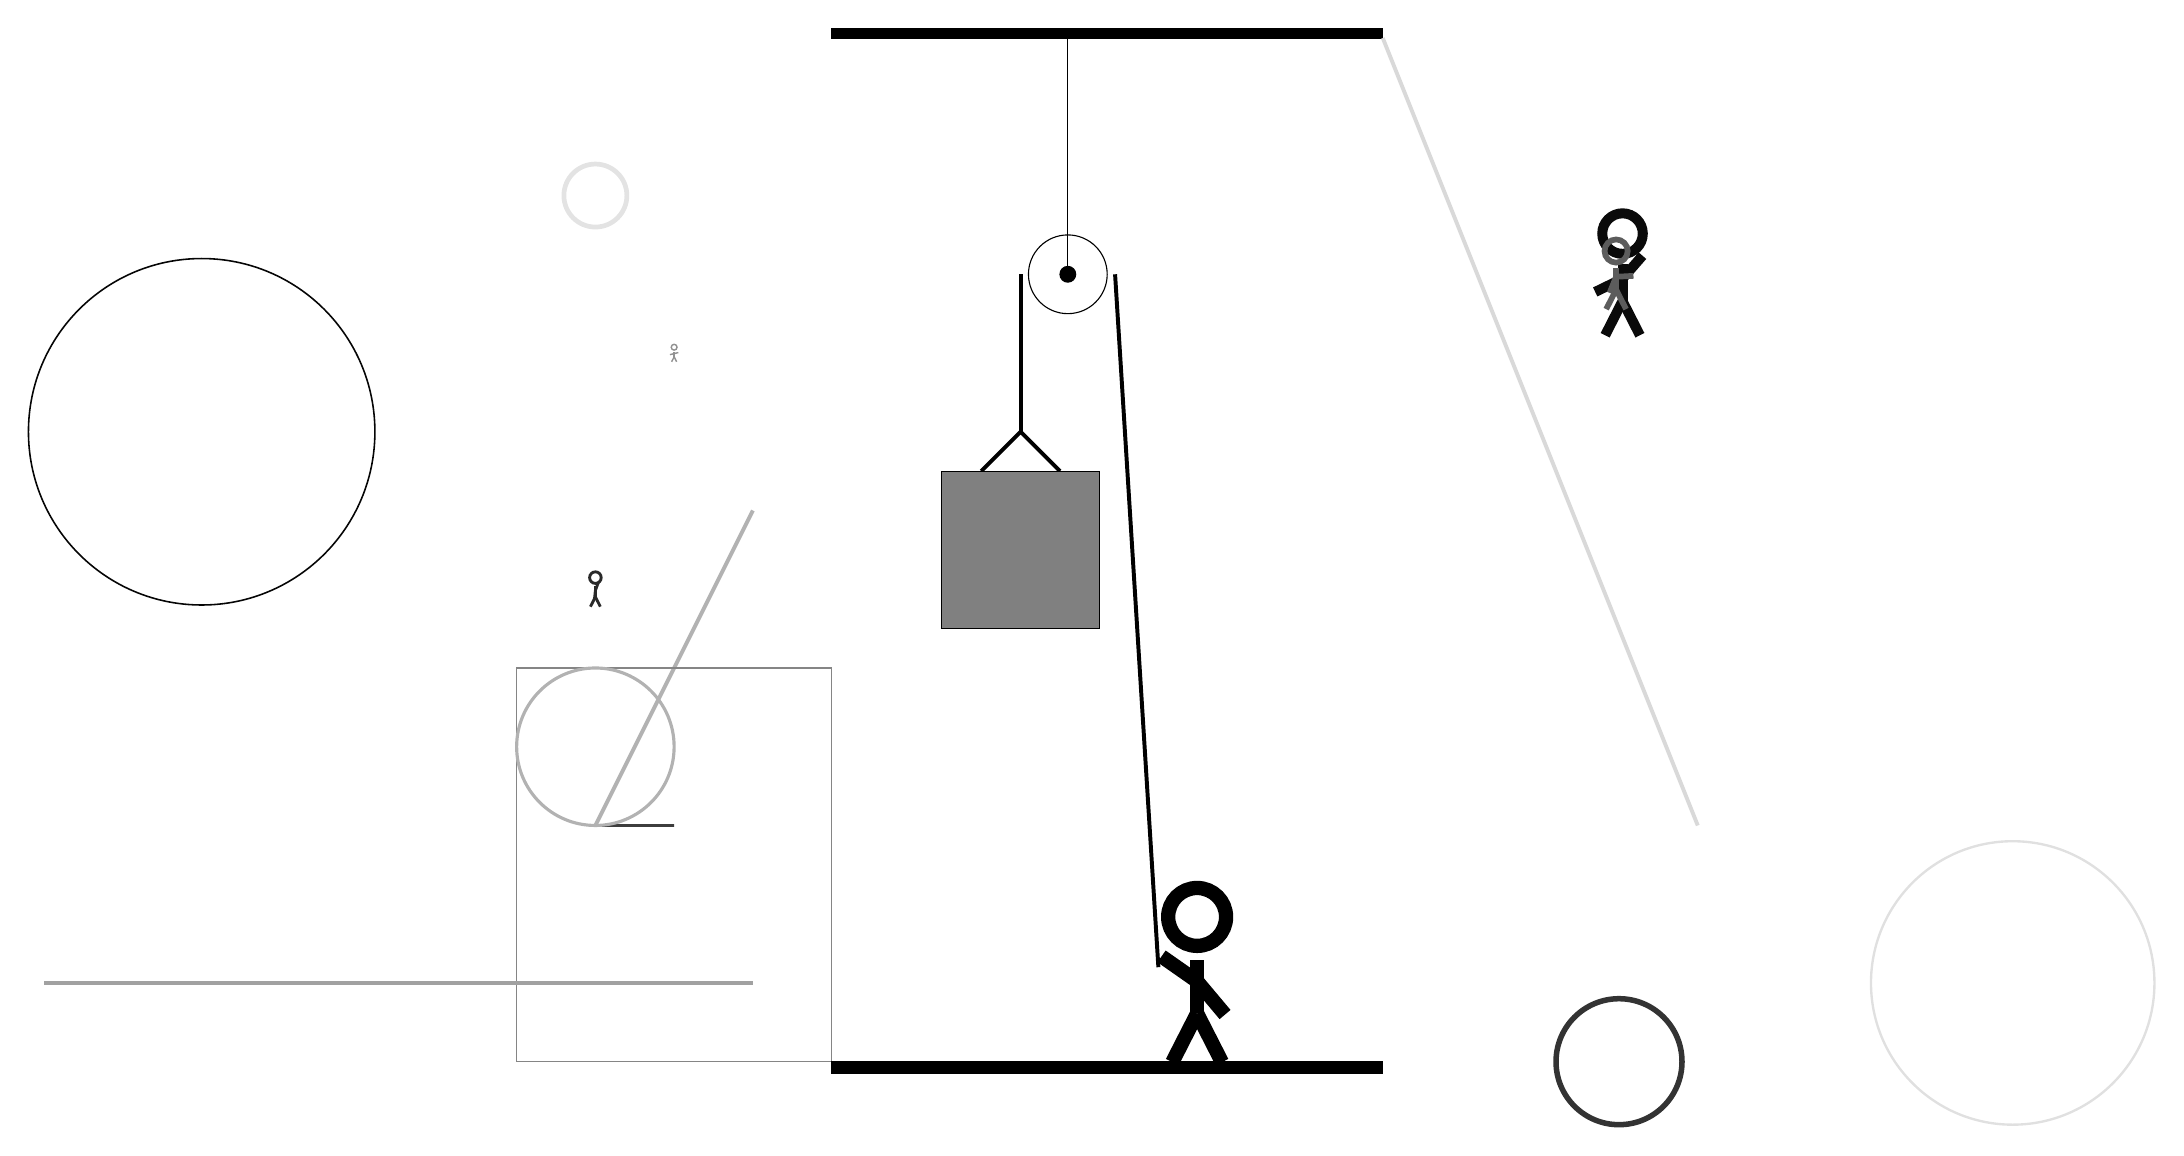
\begin{tikzpicture}
		%%%%% START %%%%%
		
		\draw[fill=black] (-2, 10) rectangle (5, 10.125);
		
		\draw (1, 7) circle (0.5);
		\draw[fill=black] (1, 7) circle (0.1);
		\draw (1, 10) -- (1, 7);
		
		\draw[line width=0.5mm] (-0.1, 4.5) -- (0.4, 5.0) -- (0.9, 4.5);
		\draw[fill=black!50] (-0.6, 4.5) rectangle (1.4, 2.5);
		
		\draw[line width=0.5mm] (0.4, 7) -- (0.4, 5.0);
		\centerarc[line width=0.5mm](1, 7)(0:180:0.6);
		\draw[line width=0.5mm](1.6, 7) -- (2.15, -1.8);
		
		\node at (2.6, -1.9) {\Strichmaxerl[10][-35][-50]};
		
		\draw [line width=0.7mm, color=black!80](8, -3) circle (0.8);
		
		\node[line width=0.4mm, color=black!43] at (-4, 6) {\Strichmaxerl[1][13][15]};
		\draw[line width=0.5mm, color=black!30](-5, 0) -- (-3, 4);
		\draw[line width=0.2mm, color=black!48] (-2, -3) rectangle (-6, 2);
		\node[line width=0.7mm, color=black!84] at (-5, 3) {\Strichmaxerl[2][84][70]};
		
		\draw[line width=0.5mm, color=black!15](9, 0) -- (5, 10);
		
		\draw [line width=0.3mm, color=black!12](13, -2) circle (1.8);
		
		\draw[line width=0.3mm, color=black!76] (-4, 0) rectangle (-5, 0);
		\draw [line width=0.4mm, color=black!30](-5, 1) circle (1.0);
		\draw [line width=0.6mm, color=black!11](-5, 8) circle (0.4);
		
		\draw[line width=0.5mm, color=black!37](-3, -2) -- (-12, -2);
		\draw [line width=0.2mm, color=black!98](-10, 5) circle (2.2);
		\node[line width=0.5mm, color=black!96] at (8, 7) {\Strichmaxerl[7][26][49]};
		\node[line width=0.4mm, color=black!64] at (8, 7) {\Strichmaxerl[4][68][3]};
		
		\draw[fill=black] (-2, -3) rectangle (5, -3.15);
		
		%%%%% END %%%%%
	\end{tikzpicture}
\end{document}